\chapter{Unsupervised learning}{I don't know what I wanna know.}
\label{chapUnsupervisedLearning}

Sometimes we observe phenomena without a precise idea in mind of what we want to investigate. Phenomena may retain information and hidden data patterns that we have never considered. Unsupervised learning use algorithms to uncover these patterns and create knowledge from the data.\footnote{The package logproj provides methods to deal with time unsupervised learning \href{https://github.com/aletuf93/logproj/blob/master/logproj/ml_unsupervised_models.py}{here}.} 

\section{Association rules} \label{secAssociationRules}
Association rules are a powerful data mining set of algorithm aiming at investigating patterns in the co-occurrences of items in a series of independent observations. Usually, they are used to mine a commercial database investigating patterns in the buyers’ attitude to set promotions, discounts or the shelf allocation. The most used algorithm is the \textit{apriori} algorithm which aims at the definition of association rules between the $p$ features of a dataset $X$.\par

The definition of association rules is based on the evaluation of the following metrics for each association rule:
\begin{itemize}
    \item Support, $T\left(p1\rightarrow\ p2\right)$. It indicates the probability that an observation contains a group of features (e.g., $(p1,\ p2)$);
    \item 	Confidence $C\left(p1\rightarrow p2\right)=\frac{T\left(p1\rightarrow\ p2\right)}{T(p1)}$, it indicates the probability a feature $p2$ is in a transaction containing $p1$ (conditional probability). It is calculated as the support of the rule divided by the support of the antecedent;
    \item 	Lift $L\left(p1\rightarrow p2\right)=\frac{C\left(p1\rightarrow p2\right)}{T(p2)}$, defines the increase in the observation of $p2$ when $p1$ is observed. 
\end{itemize}

The outcome of the $apriori$ algorithm is a set of rules $(p1\rightarrow p2)$ with support and confidence above a predetermined threshold.


\section{Clustering} \label{secClustering}
Association rules produce a list of causal relations between the features. Differently, clustering produces a label for each of the $N$ observation identifying “homogeneous” groups. Clustering, in fact, involves a set of unsupervised learning algorithms aiming at grouping the observations into subsets such that the observations in the same subset are close to each other. \par
Clustering algorithms works using proximity matrices, defining the pairwise distance between observations. For this reason, it is necessary to convert qualitative, ordinal and categorical variables such that a measure of distance is defined. \par
Hard clustering algorithm creates clusters and assigns observations to one of them; on the other side, soft clustering defines a probability for each observation to belong to each cluster. Clustering approaches are divided into:
\begin{enumerate}
    \item combinatorial algorithms, which directly works on the observed data;
    \item mixture models, which makes assumptions on the probability distributions generating the observations.
\end{enumerate}

Combinatorial algorithms (e.g., k-means) are hard-clustering algorithms minimising a loss function describing the distance between the observations. Let $k=1,\ldots,K$ be the number of clusters and $k=C(i)$ the assignment of observations $i$ to the cluster $k$. Then:

\begin{equation}
W\left(C\right)=\frac{1}{2}\sum_{k=1}^{K}\sum_{C\left(i\right)=k}\sum_{C\left(i^\prime\right)=k}{d(x_i,x_{i^\prime})}
\label{eq_clustering1}
\end{equation}

\begin{equation}
B\left(C\right)=\frac{1}{2}\sum_{k=1}^{K}\sum_{C\left(i\right)=k}\sum_{C\left(i^\prime\right)\neq k}{d(x_i,x_{i^\prime})}
\label{eq_clustering2}
\end{equation}

Where $d(x_i,x_{i^\prime})$ is the distance between data points $x_i$, and $x_{i'}$. $W(C)$ defines the distance of points within a cluster, while $B(C)$ defines the distance of points between different clusters. Combinatorial algorithms aim at maximising $W(C)$ or minimising $B(C)$. These two objectives are exactly the same.


\subsection{K-means} \label{secKmeans}
K-means algorithm is used to cluster a set of $N$ observation with $p$ features (i.e., placed in a $R^p$). This space is assumed to be Euclidean, and the algorithm produces $k$ clusters. Algorithm \ref {algo_kmeans} illustrates the procedure to generate the clusters.

\begin{algorithm}[H]
    \DontPrintSemicolon
    \SetAlgoLined
    $k=$number of centroids (clusters)\;
    $r=$number of iterations of the algorithm\;
    $i=1,...,N \in V$ set of points \;
    $j=1,...,k \in C$ set of centroids \;
    $D_i \in R^p $ set of coordinates of point i \;
    $S= \emptyset $ \;
    \For{$l=1:r$}{
    randomly assign $D_j, j\in C$\;
    $t=0$\;
    $converge=$false\;
    \While{(not $converge$)}
    {
    $t=t+1$ \;
    $z_{i,t} = argmin_{j\in C}[dist(D_j,D_i)]$ \;
    $D_j=\frac{1}{|D_i|}\sum_{z_i=j}^{}{D_i}$ \;
    \If{($z_{i,t}==z_{i,t-1}$)}
            {$converge=$true\;}
            
    }
    $z = \sum_{i=1}^{N}{\sum_{j=1}^{k}{dist[(D_j,D_i)]}}$ \;
    $S=S \bigcup z$
    }
    Select $min(z) \in S$ \;

\caption{K-means algorithm}
\label{algo_kmeans}    
\end{algorithm}

We use the \textit{digits dataset} containing images of a digit to show the power of unsupervised learning techniques. The dataset contains images of digits, from zero to nine with their label. We use unsupervised learning to cluster the observations, and we project the input dataset into two components to visually compare the results of the clustering with the true label. Figure \ref{fig_kmeans} illustrates that k-means is able to detect patterns similar to the true labels.\footnote{The source code of Figure \ref{fig_kmeans} is available \href{https://github.com/aletuf93/logproj/blob/master/examples/06.\%20Unsupervised\%20learning.ipynb}{here}.
}

% INSERT fig_kmeans
\begin{figure}[hbt!]
\centering
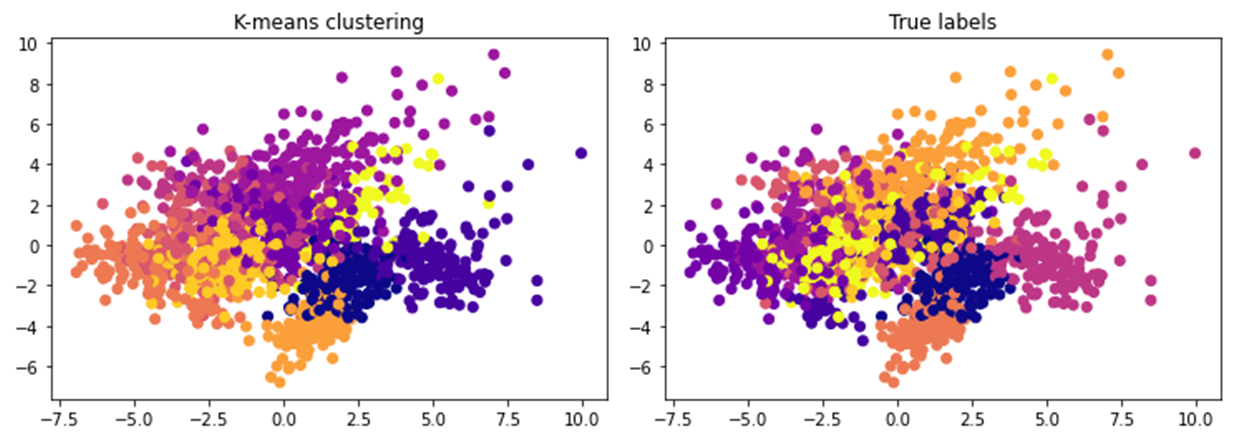
\includegraphics[width=0.9\textwidth]{SectionLetsMath/unsupervisedLearning_figures/fig_kmeans.png}
\captionsetup{type=figure}
\caption{Comparison between k-means clustering and true labels of the digits dataset. Different colours identify different labels. There is no specific assignment between colours and labels.}
\label{fig_kmeans}
\end{figure}

\subsection{Hierarchical clustering} \label{secHierarchicalClustering}
Hierarchical clustering defines clusters based on a proximity metric between the observations. Similarly to Multi-Dimensional scaling (see Section \ref{secMultiDimensionalScaling}) hierarchical clustering does not work with a matrix $X_{N,P}$ with  a number of observations $N$ and $P$ features (as the k-means algorithm does). Hierarchical clustering relies on a proximity matrix $D_{N,N}$ expressing a pairwise distance between each observation (according to a single feature expressing a distance).  It is common to work using similarity values $s_{ij}$ as entries of $D_{N,N}$. Once the pairwise distance $d_{i,j}$ is calculated, the similarity can be calculated as $s_{i,j}=1-\frac{d_{i,j}}{\max_{i,j}{d_{i,j}}}$. Table \ref{tab_similarityMatrix} illustrates an example of the proximity matrix $D_{N,N}$.

% INSERT tab_similarityMatrix
\begin{figure}[hbt!]
\centering
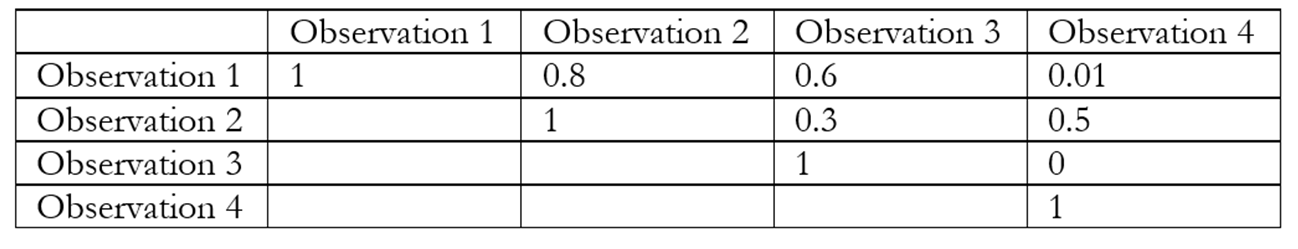
\includegraphics[width=0.9\textwidth]{SectionLetsMath/unsupervisedLearning_figures/tab_similarityMatrix.png}
\captionsetup{type=table}
\caption{Example of a similarity matrix.}
\label{tab_similarityMatrix}
\end{figure}

The matrix in Table \ref{tab_similarityMatrix} is symmetric, this is not strictly required, but it can simplify the structure of the data without adding too much bias. If a similarity matrix is not symmetric, it can be converted into a symmetric one by setting $s_{i,j}=s_{j,i}=\frac{s_{i,j}+s_{j,i}}{2}$. Once $D_{N,N}$ is defined, it is possible to apply hierarchical clustering to group the N observations into clusters. The number of clusters is not defined in advance. Algorithm \ref{algo_hierarchical} presents an algorithm for hierarchical clustering.

\begin{algorithm}[H]
\DontPrintSemicolon
\SetAlgoLined
    
    $i=1,...,N \in V$ set of observations \;
    
    $s_{i,j}$ similarity between observation i and j \;
    
    $S= \emptyset $ \;
    \For{$k \leftarrow 1:(N-1)$}
    {
    $v =\max_{(i,j)-S}{(s_{i,j})}$ \;
    $(h,l)=\arg(v)$\;
    $S= S \bigcup (h,l)$ \;
    \For{$r \leftarrow 1: m$}
    {
    \If{CLINK} {
    $s_{r,h}=min(s_{r,h},s_{r,l})$\;
    $s_{h,r}=min(s_{h,r},s_{l,r})$\;
    }
    \If{SLINK} {
    $s_{r,h}=max(s_{r,h},s_{r,l})$\;
    $s_{h,r}=max(s_{h,r},s_{l,r})$\;
    }
    \If{UPGMA} {
    $s_{r,h}=mean(s_{r,h},s_{r,l})$\;
    $s_{h,r}=mean(s_{h,r},s_{l,r})$\;
    }
    $s_{r,l}=-1$\;
    $s_{l,r}=-1$\;
    
    }
    }
\caption{Hierarchical clustering algorithm}
\label{algo_hierarchical}        
\end{algorithm}

The algorithm iteratively selects two observations and aggregate them into a single cluster until all the observations belong to one big cluster. The value of similarity $s_{i,j}$ of an observation $i$ (aggregated with an observation $k$ at an iteration) and all the others, $j$ is selected according to the tuning of the algorithm which can consider the minimum, the maximum or the average (complete linkage, single linkage or average linkage) among $s_{i,j}$ and $s_{k,j}$.\par

Since each observation/cluster is aggregated at a value of similarity, at the end of the procedure, a similarity threshold is selected to identify a number of clusters and the cluster each observation belongs. This procedure can be visually interpreted by a dendrogram which maps the aggregations of the algorithms with a threshold of similarity identifying the clusters. Figure \ref{fig_dendrograms} illustrates the dendrogram obtained clustering the digits dataset using single, complete and average linkages having a Euclidean distance between the observations.\footnote{The source code of Figure \ref{fig_dendrograms} is available \href{https://github.com/aletuf93/logproj/blob/master/examples/06.\%20Unsupervised\%20learning.ipynb}{here}.}

% INSERT fig_dendrograms
\begin{figure}[hbt!]
\centering
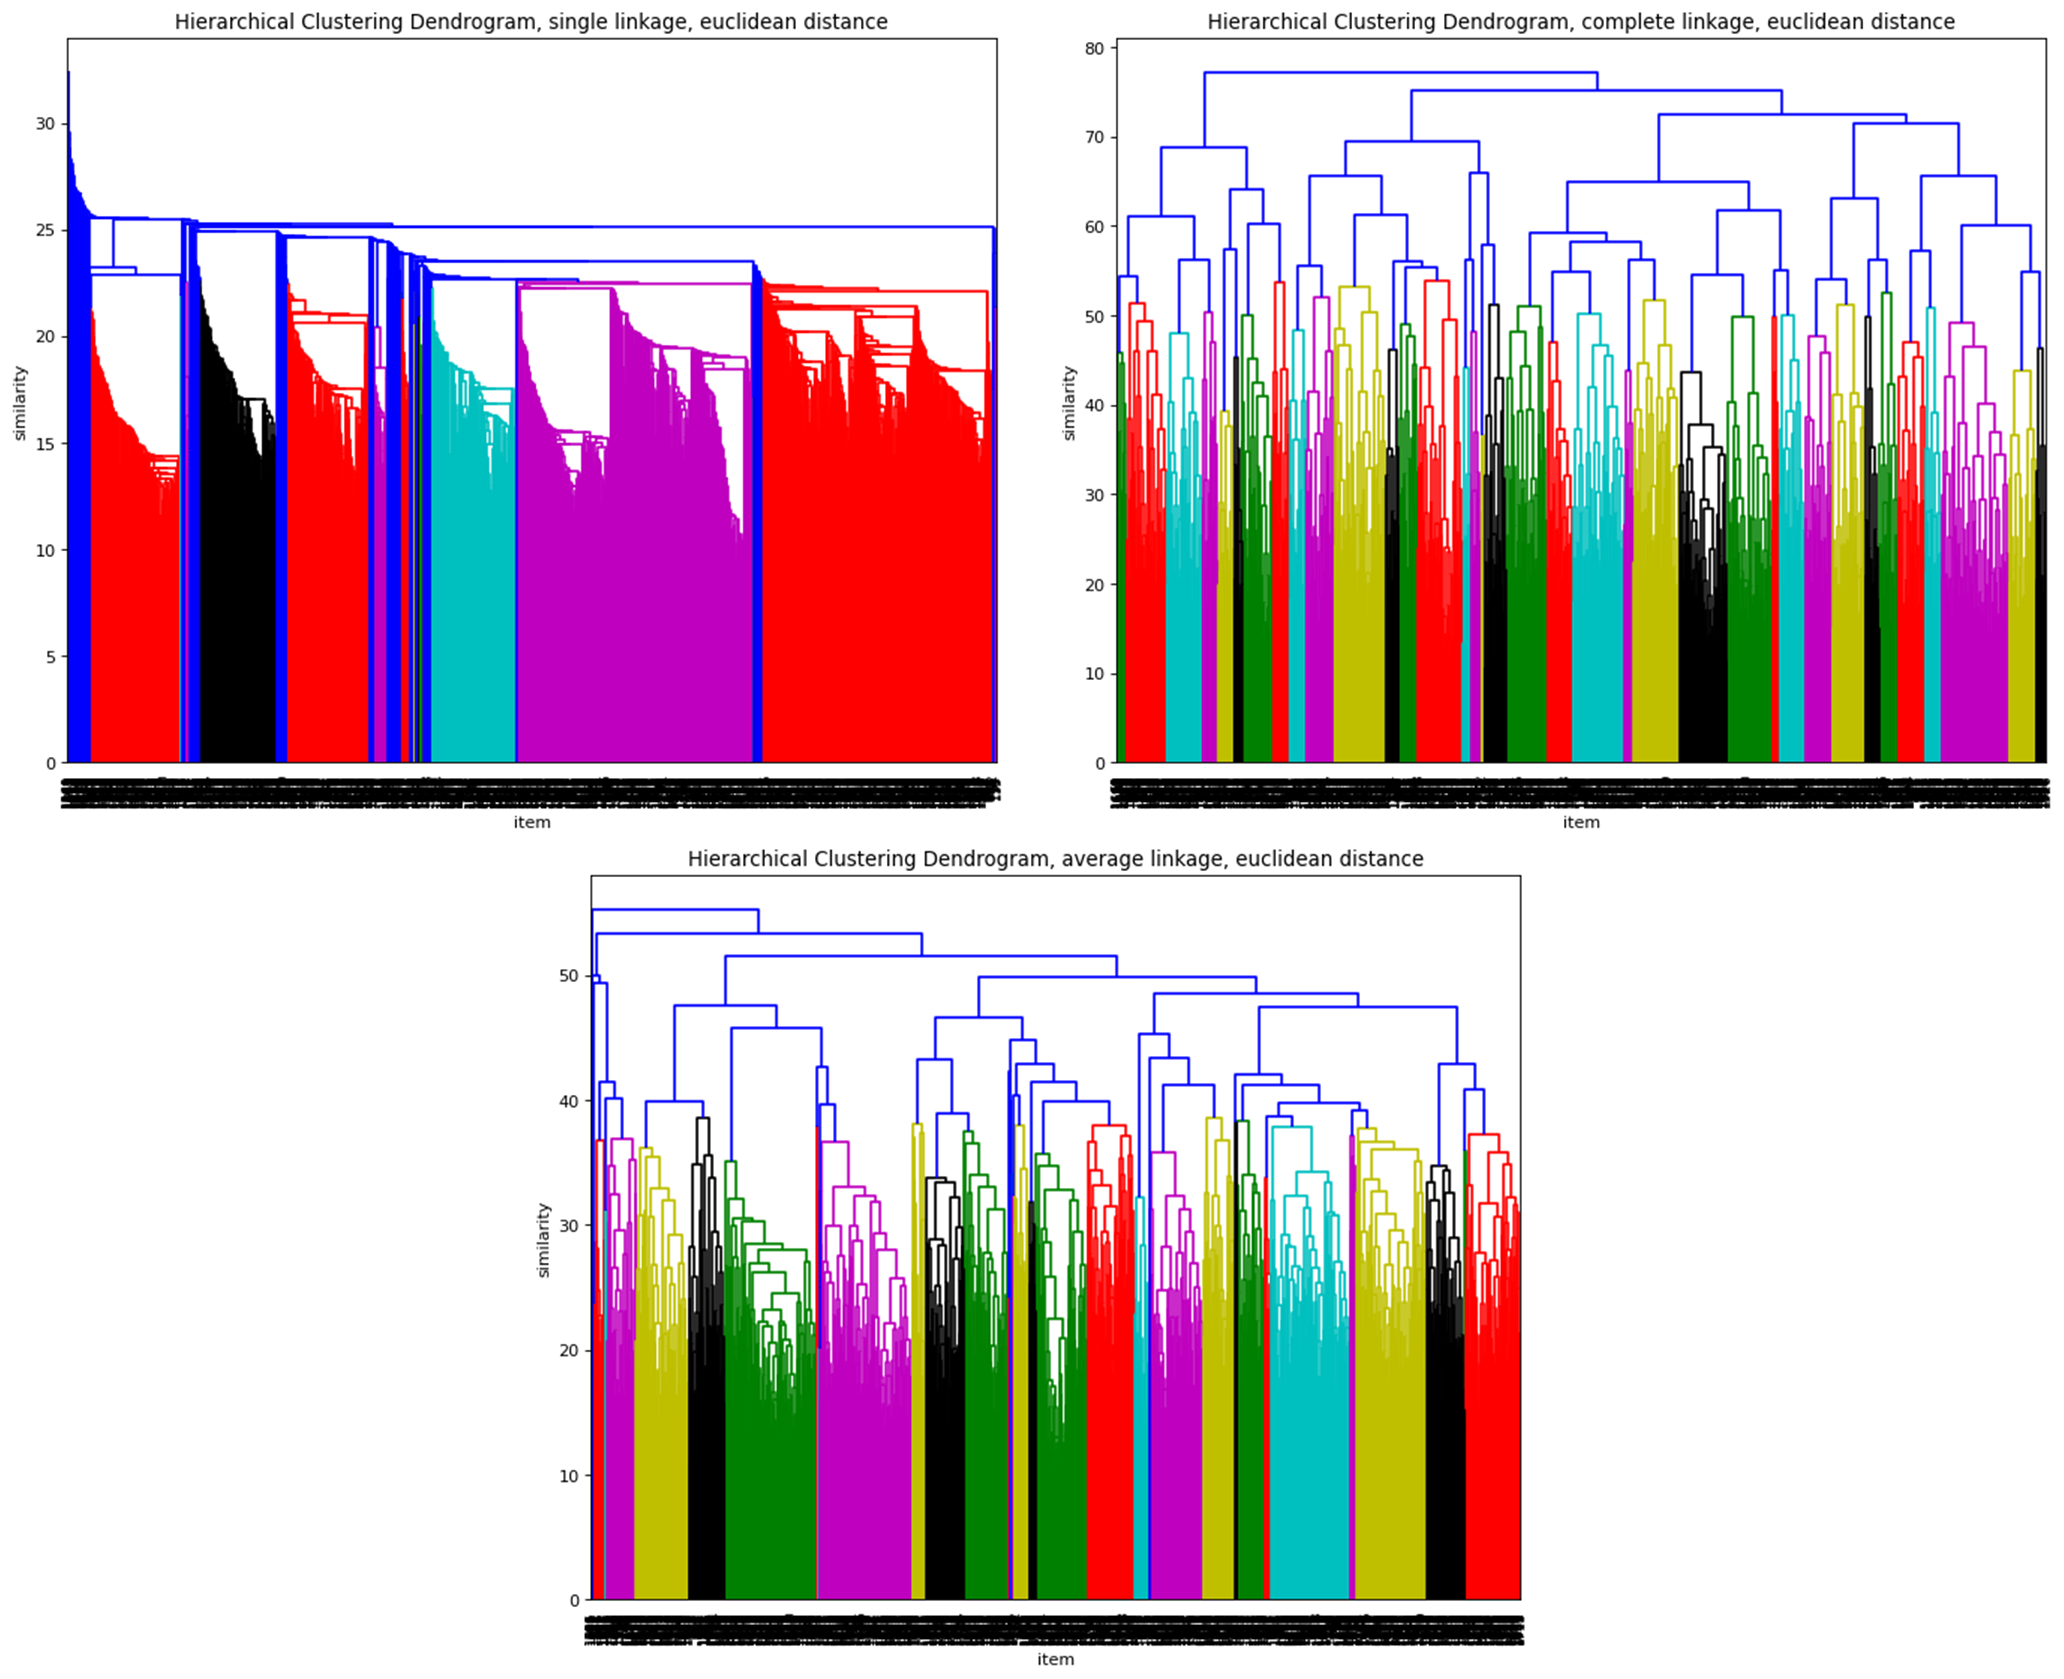
\includegraphics[width=0.9\textwidth]{SectionLetsMath/unsupervisedLearning_figures/fig_dendrograms.png}
\captionsetup{type=figure}
\caption{Similarity dendrograms of the digits dataset.}
\label{fig_dendrograms}
\end{figure}

Different similarity thresholds identify a different number of clusters. Assuming ten clusters, ad the number of labels of the digits dataset, Figure \ref{fig_hierarchical} illustrates the comparison between the clusters obtained with the different linkages and the true labels.\footnote{The source code of Figure \ref{fig_hierarchical} is available \href{https://github.com/aletuf93/logproj/blob/master/examples/06.\%20Unsupervised\%20learning.ipynb}{here}.}

% INSERT fig_hierarchical
\begin{figure}[hbt!]
\centering
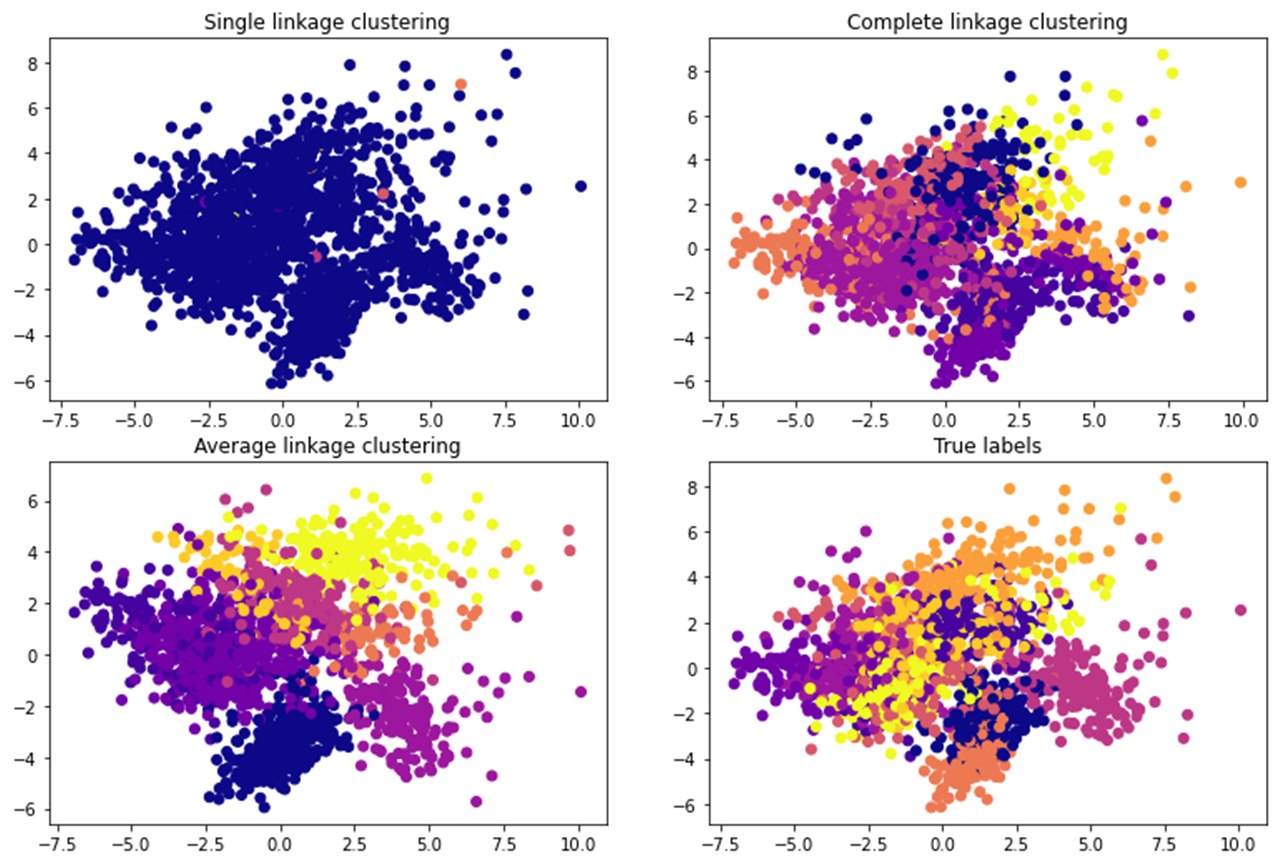
\includegraphics[width=0.9\textwidth]{SectionLetsMath/unsupervisedLearning_figures/fig_hierarchical.png}
\captionsetup{type=figure}
\caption{Comparison between hierarchical clustering and true labels of the digits dataset. Different colours identify different labels. There is no specific assignment between colours and labels.}
\label{fig_hierarchical}
\end{figure}

\subsection{Mixture models} \label{secGaussianMixture}
In general, the observations may be generated by an unknown number K of PDF with unknown parameters (i.e. mean and variance). Mixture models are soft clustering techniques used to investigate the probability that a point is generated by one of the K generating PDF. It is called soft because it defines a probability for each point and each distribution, without a direct binary (i.e. true or false) assignment to a cluster. The generating function of a Gaussian mixture model can be seen as:

\begin{equation}
f\left(x\right)=\sum_{m=1}^{K}{\alpha_m\phi(x;\mu_m;\Sigma_m})
\label{eq_gmm}
\end{equation}

Where $\phi$ is a multidimensional Gaussian PDF with parameters $\mu_m$ and $\Sigma_m$, and $\alpha_m\in[0,1]$ is the probability of the $m$-th generating function. The problem of fitting a mixture model to data is to define the value of $\alpha_m$, $\mu_m$, $\Sigma_m$ that best represent the real distribution of the data. This is a likelihood maximisation problem with $\theta=\alpha_m$,$\mu_m$,$\Sigma_m$. To efficiently get the result the so-called EM-algorithm (Expectation-Maximization) is used. This algorithm can be used when it is difficult to maximise a likelihood but it is made simpler by enlarging the sample using unobserved data. Considering K=2, the EM algorithm can be exemplified as follows:

\begin{algorithm}[H]
\DontPrintSemicolon
\SetAlgoLined
    
    1. Randomly select $\mu_a,\sigma_a,\mu_b,\sigma_b$ \;
    2. Calculate the posterior probability $a_i=Prob(a|x_i)$ and $b_i=Prob(b|x_i)$ \;
    3. Redefine $\mu_a,\sigma_a,\mu_b,\sigma_b$ as the weighted average of mean and variance of $x_i$ in $a$ and $b$ \;
    4. Repeat from 2. until $\mu_a,\sigma_a,\mu_b,\sigma_b$ converges\;
    
    
    
   
\caption{Expectation Maximization (EM) algorithm}
\label{algo_EM}        
\end{algorithm}

Figure \ref{fig_gmm} illustrates the output of a Gaussian mixture model applied to the digits dataset.\footnote{The source code of Figure \ref{fig_gmm} is available \href{https://github.com/aletuf93/logproj/blob/master/examples/06.\%20Unsupervised\%20learning.ipynb}{here}.}

% INSERT fig_gmm
\begin{figure}[hbt!]
\centering
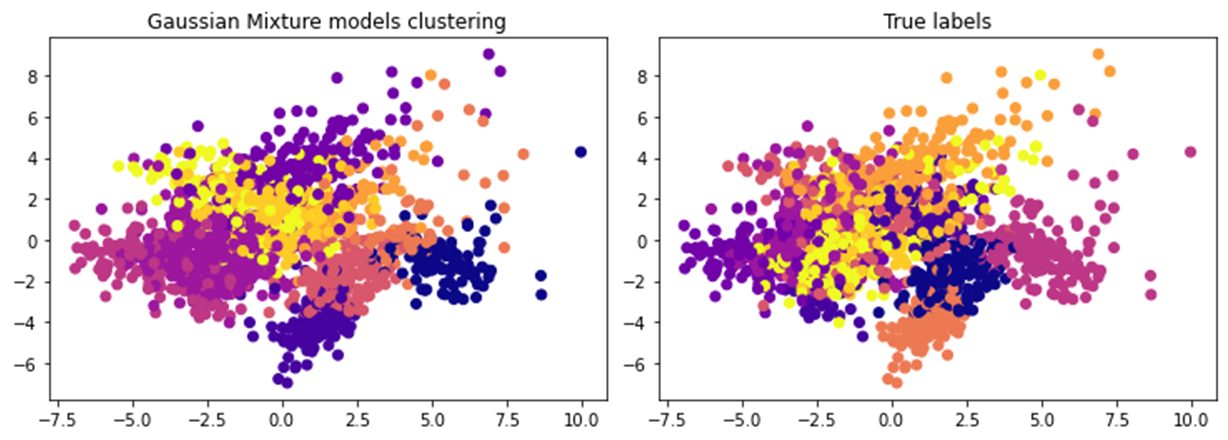
\includegraphics[width=0.9\textwidth]{SectionLetsMath/unsupervisedLearning_figures/fig_gmm.png}
\captionsetup{type=figure}
\caption{Comparison between Gaussian mixture model and true labels of the digits dataset. Different colours identify different labels. There is no specific assignment between colours and labels.}
\label{fig_gmm}
\end{figure}

\subsection{Bag of words} 
A Bag of words is a text-mining method which works as an unsupervised model for strings. It is a frequency analysis for strings of text. Given a dataset composed of $N$ strings (e.g., a paragraph) the bag of word model counts the number of occurrences of each string. Each string can be interpreted as a feature of the dataset with different relative importance. The words occurring the most retain the highest level of information of the dataset and can be used as predictors (e.g., depending on the content, it is possible to classify an email into spam/not spam).



\section*{Further reading}
Supplementary reading materials can be found in \cite{Aggarwal2015}, \cite{Blattberg2008}.

%\clearpage
\bibliographystyle{ieeetr}
\bibliography{SectionLetsMath/unsupervisedLearning_ref}



